\chapter{Psalm 45}

\begin{figure}
  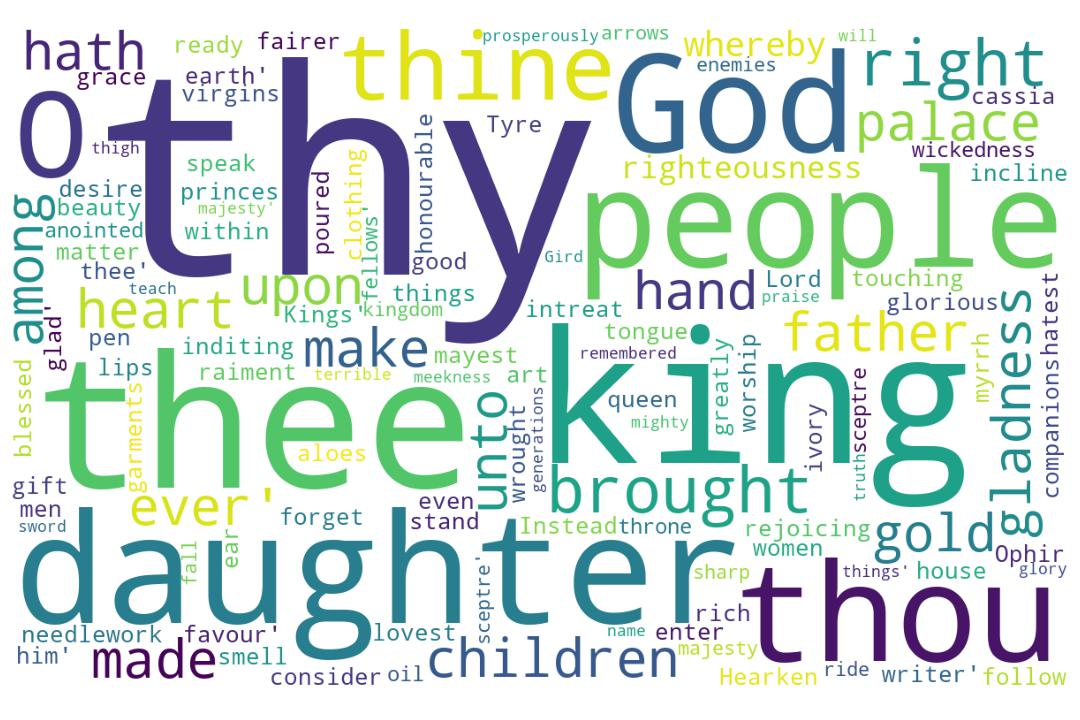
\includegraphics[width=\linewidth]{19OT-Psalms/Psalm45-WordCloud.jpg}
  \caption{Psalm 45 Word Cloud}
  \label{fig:Psalm 45 word Cloud}
\end{figure}

\marginpar{\scriptsize \centering \fcolorbox{bone}{lime}{\textbf{THE WEDDING SCENE}}\\ (Psalm 45:1-17) \begin{compactenum}[I.][8]
    \item A \textbf{Great Husband} \index[scripture]{Psalms!Psa 045:02}(Psa 45:2)
    \item \textbf{Glory \& } \index[scripture]{Psalms!Psa 045:08}(Psa 45:8)
    \item \textbf{Gladness \& Happiness} \index[scripture]{Psalms!Psa 045:07}(Psa 45:7)
    \item The \textbf{Groom is Here} \index[scripture]{Psalms!Psa 045:08}(Psa 45:8)
    \item The \textbf{Guests on High} (one theologian argues -- and I agree -- that the wedding guests will include believers from all ages, such as those before the Law, Gentile believers during the Law, etc -- all there to witness the Lord and His bride)\index[scripture]{Psalms!Psa 045:08}(Psa 45:8)
    \item \textbf{Gifts handed over} \index[scripture]{Psalms!Psa 045:12}(Psa 45:12)
    \item The \textbf{Gown and Handmaidens} \index[scripture]{Psalms!Psa 045:14}(Psa 45:14)
\end{compactenum}}

\footnote{\textcolor[cmyk]{0.99998,1,0,0}{\hyperlink{TOC}{Return to end of Table of Contents.}}}\footnote{\href{https://audiobible.com/bible/psalms_45.html}{\textcolor[cmyk]{0.99998,1,0,0}{Psalms Audio}}}\textcolor[cmyk]{0.99998,1,0,0}{To the chief Musician upon Shoshannim, for the sons of Korah, Mashil, A Song of loves}\footnote{\textbf{Revelation 19:7-10} - Let us be glad and rejoice, and give honour to him: for the marriage of the Lamb is come, and his wife hath made herself ready. [8] And to her was granted that she should be arrayed in fine linen, clean and white: for the fine linen is the righteousness of saints. [9] And he saith unto me, Write, Blessed are they which are called unto the marriage supper of the Lamb. And he saith unto me, These are the true sayings of God. [10] And I fell at his feet to worship him. And he said unto me, See thou do it not: I am thy fellowservant, and of thy brethren that have the testimony of Jesus: worship God: for the testimony of Jesus is the spirit of prophecy.}\\
\\
\textcolor[cmyk]{0.99998,1,0,0}{My heart is inditing a good matter: I speak of the things which I have made touching the king: my tongue \emph{is} the pen of a ready writer.}
[2] \textcolor[cmyk]{0.99998,1,0,0}{Thou art fairer than the children of men: grace is poured into thy lips: therefore God hath blessed thee for ever.}
[3] \textcolor[cmyk]{0.99998,1,0,0}{Gird thy sword upon \emph{thy} thigh, O \emph{most} mighty, with thy glory and thy majesty.}\footnote{\textbf{Genesis 3:24} - So he drove out the man; and he placed at the east of the garden of Eden Cherubims, and a flaming sword which turned every way, to keep the way of the tree of life.}\footnote{\textbf{Joshua 5:13-15} - And it came to pass, when Joshua was by Jericho, that he lifted up his eyes and looked, and, behold, there stood a man over against him with his sword drawn in his hand: and Joshua went unto him, and said unto him, Art thou for us, or for our adversaries? [14] And he said, Nay; but as captain of the host of the LORD am I now come. And Joshua fell on his face to the earth, and did worship, and said unto him, What saith my lord unto his servant? [15] And the captain of the LORD’S host said unto Joshua, Loose thy shoe from off thy foot; for the place whereon thou standest is holy. And Joshua did so.}\footnote{\textbf{Hebrews 4:12} - For the word of God is quick, and powerful, and sharper than any twoedged sword, piercing even to the dividing asunder of soul and spirit, and of the joints and marrow, and is a discerner of the thoughts and intents of the heart.}\footnote{\textbf{Revelation 19:15} - And out of his mouth goeth a sharp sword, that with it he should smite the nations: and he shall rule them with a rod of iron: and he treadeth the winepress of the fierceness and wrath of Almighty God.}\footnote{\textbf{Revelation 19:21} - And the remnant were slain with the sword of him that sat upon the horse, which sword proceeded out of his mouth: and all the fowls were filled with their flesh.} 
[4] \textcolor[cmyk]{0.99998,1,0,0}{And in thy majesty ride prosperously because of truth and meekness \emph{and} \fcolorbox{bone}{MYGOLD}{righteousness}; and thy right hand shall teach thee terrible things.}
[5] \textcolor[cmyk]{0.99998,1,0,0}{Thine arrows \emph{are} sharp in the heart of the king's enemies; \emph{whereby} the people fall under thee.}
[6] \textcolor[cmyk]{0.99998,1,0,0}{Thy throne, O God, \emph{is} for ever and ever: the sceptre of thy kingdom \emph{is} a right sceptre.}
[7] \textcolor[cmyk]{0.99998,1,0,0}{Thou lovest \fcolorbox{bone}{MYGOLD}{righteousness}, and hatest wickedness: therefore God, thy God, hath anointed thee with the oil of gladness above thy fellows.}
[8] \textcolor[cmyk]{0.99998,1,0,0}{All thy garments \emph{smell} of myrrh, and aloes, \emph{and} cassia, out of the ivory palaces, whereby they have made thee glad.}
[9] \textcolor[cmyk]{0.99998,1,0,0}{Kings' daughters \emph{were} among thy honourable women: upon thy right hand did stand the queen in gold of Ophir.}
[10] \textcolor[cmyk]{0.99998,1,0,0}{Hearken, O daughter, and consider, and incline thine ear; forget also thine own people, and thy father's house;}
[11] \textcolor[cmyk]{0.99998,1,0,0}{So shall the king greatly desire thy beauty: for he \emph{is} thy Lord; and worship thou him.}
[12] \textcolor[cmyk]{0.99998,1,0,0}{And the daughter of Tyre \emph{shall} \emph{be} \emph{there} with a gift; \emph{even} the rich among the people shall intreat thy favour.}
[13] \textcolor[cmyk]{0.99998,1,0,0}{The king's daughter \emph{is} all glorious within: her clothing \emph{is} of wrought gold.}
[14] \textcolor[cmyk]{0.99998,1,0,0}{She shall be brought unto the king in raiment of needlework: the virgins her companions that follow her shall be brought unto thee.}
[15] \textcolor[cmyk]{0.99998,1,0,0}{With gladness and rejoicing shall they be brought: they shall enter into the king's palace.}
[16] \textcolor[cmyk]{0.99998,1,0,0}{Instead of thy fathers shall be thy children, whom thou mayest make princes in all the earth.}
[17] \textcolor[cmyk]{0.99998,1,0,0}{I will make thy name to be remembered in all generations: therefore shall the people praise thee for ever and ever.}

